\documentclass[11pt, a4paper]{article}

% -- Packages ------------------------------------------------------------------
\usepackage[utf8]{inputenc}
\usepackage[T1]{fontenc}
\usepackage{lmodern}
\usepackage[margin=2.5cm]{geometry}
\usepackage{amsmath, amssymb, amsthm}
\usepackage{graphicx}
\usepackage{tikz}
\usepackage{xcolor}
\usepackage{microtype}
\usepackage{parskip}
\usepackage[above,below]{placeins}
\usepackage{hyperref}

\hypersetup{colorlinks=true, linkcolor=black, citecolor=teal, urlcolor=teal}

\newcommand{\R}{\mathbb{R}}
\newcommand{\vOS}{\textsf{vOS}}
\newcommand{\nucleus}{\texttt{vsf-nucleus}}

% -- Title ----------------------------------------------------------------------
\title{%
  \textbf{Geometric Attractor Convergence in a Viable System Kernel}\\[4pt]
  \large Executive Summary
}

\author{Luis Pineda R.\thanks{Contact: \texttt{luis@tallerpineda.cl}}}
\date{\textit{Technical Report -- April 2026; revised June 2026}}

\begin{document}
\maketitle

% ??????????????????????????????????????????????????????????????????????????????
\section*{What We Did}

We built a computational kernel (\nucleus{}) based on Beer's Viable System Model
(VSM) and tested whether a system governed by a small set of cybernetic axioms
converges to a stable attractor in state space. The kernel's state is a point in
$\R^{128}$, structured into semantic blocks: identity, resources, entropy,
operations, communication channels, attractor memory, and regulatory intelligence.

We ran twelve experiments on physical hardware (Intel Core i7-7600U, Proxmox
hypervisor) from April 2026 onward, measuring convergence, basin geometry, thermal
resilience, observer effects, architecture ablation, and --- in the final experiment
--- the whole assembled system with every VSM layer running live.

% ??????????????????????????????????????????????????????????????????????????????
\section*{Headline Results}

\textbf{1. The attractor is a stable point sink, confirmed three independent ways.}
We measured the largest Lyapunov exponent directly (Benettin's method):
$\lambda_\text{max} = -0.010050 = \ln(0.99)$ per tick, to machine precision ---
negative, so nearby trajectories contract rather than diverge. A Monte-Carlo
estimate puts the basin volume at $\approx 1.0$ over the reachable region, and
persistent-homology topology gives $\beta_0 = 1,\ \beta_1 = 0$ (one component, no
hole, no limit cycle). Dynamics, volume, and shape agree: a single stable point.

\textbf{2. A coordinate-free viability certificate, $V = \min(g, c, t, m)$.}
We distil the measurements into one functional built from intrinsic invariants
(feasibility, contraction sign, topological signature, noise margin). On this kernel
the binding axis is $g = 0.102$ (the CPU-budget constraint), and breaking any single
axis independently drives $V \to 0$ --- so $V$ is a discriminating vector, not a
cosmetic scalar that is always near one.

\textbf{3. The observer is constitutive, not passive.} Structured observation
measurably lowers the system's entropy by $0.31$ bits and compresses its effective
dimension from $\approx 5.0$ to $3.9$ --- a measured instance of second-order
cybernetics, where the observer is part of the dynamics it stabilises.

% ??????????????????????????????????????????????????????????????????????????????
\section*{Key Finding: Two-Layer Viability}

The ablation experiments reveal a \textbf{two-layer viability structure}:

\begin{figure}[h]
\centering
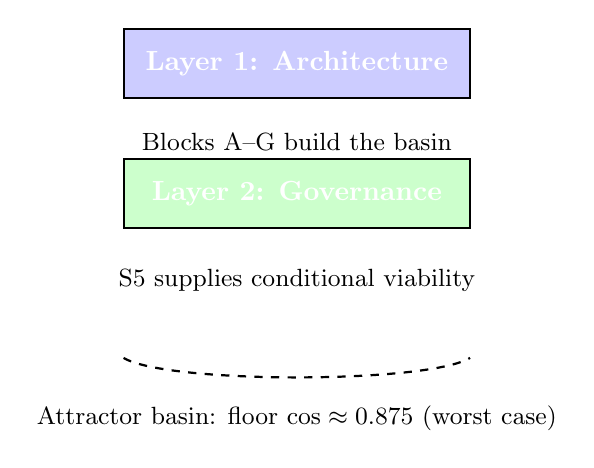
\begin{tikzpicture}[scale=1.1]
  \draw[thick, fill=blue!20] (0,3) rectangle (4,3.8);
  \node at (2,3.4) [text=white, font=\bfseries] {Layer 1: Architecture};
  \node at (2,2.5) {\small Blocks A--G build the basin};

  \draw[thick, fill=green!20] (0,1.5) rectangle (4,2.3);
  \node at (2,1.9) [text=white, font=\bfseries] {Layer 2: Governance};
  \node at (2,0.9) {\small S5 supplies conditional viability};

  \draw[dashed, thick] (0,0) .. controls (0.5,-0.3) and (3.5,-0.3) .. (4,0);
  \node at (2,-0.7) {\small Attractor basin: floor $\cos \approx 0.875$ (worst case)};
\end{tikzpicture}
\caption{Architecture builds the basin and its homeostasis; governance is the
difference between survival and collapse under stress.}
\label{fig:two_layer}
\end{figure}

\begin{description}
  \item[\textbf{Layer 1: Architecture}] The arrangement of VSM blocks physically
        determines which regions of state space are habitable. The bare substrate
        (no blocks) drifts off-target and never stabilises; the blocks are what
        create the $\R^{128}$ point sink.
  \item[\textbf{Layer 2: Governance (S5)}] At rest, governance is \emph{redundant}
        --- the system converges identically with or without it. Under stress it is
        decisive. Governance has two arms: a \emph{reactive} one (the algedonic
        safety response that throttles a runaway thermal load) and a
        \emph{deliberative} one (the constitutional covenant veto that can halt the
        system's own autonomy). The experiments exercise both.
\end{description}

When both layers are present the system holds viability at $\cos \approx 0.875$ (on a
$0$--$1$ scale, $0.70$ = viable threshold) even under maximum impulsive stress --- a
margin of $0.175$ never breached in any experiment.

% ??????????????????????????????????????????????????????????????????????????????
\section*{The Capstone: an Operationally Closed System}

The final experiment ran the complete kernel with all five of Beer's systems
(S1--S5) live, under a single perturbation. Each level engaged within its own
cybernetic scope. The decisive observation traverses the whole model in one tick:
operations (S1) registered a dip, coordination (S2) delivered a policy signal,
control (S3) detected the degradation and \emph{attempted} a correction, and policy
(S5) \emph{overruled} it --- after which the system self-recovered. A separate test
confirmed the constitutional veto end-to-end: it halts autonomous control under
sustained degradation and restores it only on an explicit, cryptographically
recorded human resume.

This is the point of the architecture: not a simulation of Beer's diagram, but a
system in which each arrow carries a measured event.

% ??????????????????????????????????????????????????????????????????????????????
\section*{Empirical Results}

\begin{tabular}{lrl}
\textbf{Property} & \textbf{Measure} & \textbf{Status} \\
\hline
Lyapunov exponent        & $\lambda_\text{max} = \ln(0.99) < 0$ & Measured, point sink \\
Basin volume             & $\approx 1.0$ (reachable region)     & Monte-Carlo \\
Topology                 & $\beta_0 = 1,\ \beta_1 = 0$          & No limit cycle \\
Basin uniqueness         & $\cos_\text{mean pairwise} = 0.9854$ & Confirmed \\
Thermal viability        & viable at $68\,^\circ\mathrm{C}$     & Holds \\
Basin floor (impulsive)  & $\cos \approx 0.875$                 & Margin $0.175$ \\
Observer entropy drop    & $\Delta H = 0.31$ bits               & Constitutive \\
Viability certificate    & $V = \min(g,c,t,m),\ g = 0.102$      & Discriminates \\
Real-process governance  & 4 OS processes, $\tau = 1.0$         & cgroup~v2 live \\
VSM operational closure  & S1--S5 causal in one run             & Demonstrated \\
\end{tabular}

% ??????????????????????????????????????????????????????????????????????????????
\section*{What This Means}

\begin{enumerate}
  \item \textbf{Viability is geometric.} The system's stability emerges from the
        geometry of its state space, not from external enforcement. This is what
        Beer meant by a \emph{viable system}.

  \item \textbf{Ethical constraints enter as feasibility conditions.} The axioms
        that prohibit harm and coercion are not bolted on --- a covenant violation
        collapses viability ($V \to 0$) exactly as exhausting the CPU budget does.
        The mathematics is \emph{indifferent} to which constraints encode ethics;
        that indifference is precisely what makes it a general certifier rather than
        a moral theory.

  \item \textbf{Governance is conditional resilience.} A well-designed policy layer
        does not \emph{create} viability --- the architecture does that --- but it is
        the difference between graceful survival and collapse when the system is
        challenged.

  \item \textbf{The basin is deep.} Under every tested perturbation the system never
        approached the viability threshold ($0.70$); the nearest approach was
        $0.875$, a $12.5\%$ margin above failure.
\end{enumerate}

% ??????????????????????????????????????????????????????????????????????????????
\section*{Honest Limits}

The work runs on a single hardware node; the thermal stressor, while it drives real
silicon temperature, is a synthetic workload; and most runs are closed-system. The
final, sharpest limit is informative: because the attractor holds its viability
measure invariant even against a CPU load more than twice the core count, the
system's \emph{anticipatory} channel cannot read an early warning from its own
regulated state. Genuine anticipation requires an external environment ---
variables whose variance is independent of the kernel's own attractor. Coupling the
kernel to such an environment is the principal direction of ongoing work.

% ??????????????????????????????????????????????????????????????????????????????
\section*{Next Steps}

\begin{enumerate}
  \item \textbf{External environment coupling.} Connect the kernel to genuinely
        external operational units (the motivating case: a distributed climate-sensing
        network) whose signals are not slaved to the kernel's attractor --- the test
        the anticipatory channel actually needs.
  \item \textbf{Inter-system coordination via a formal substrate.} A companion line
        of work studies whether two heterogeneous models can coordinate as distinct
        VSM layers through a shared formal language (the basis of a second paper).
  \item \textbf{\vOS{} on bare metal.} Deploy the kernel against real workloads
        (databases, inference) to measure attractor geometry under diverse load.
\end{enumerate}

% ??????????????????????????????????????????????????????????????????????????????
\section*{For the Beer Community}

This work returns to first principles: \emph{what does it mean for a system to be
viable?} We give a computational answer grounded in cybernetic axioms, with
instruments --- Benettin's algorithm, persistent homology, cryptographic attestation
--- that did not exist when Beer wrote. The architecture--governance distinction, and
the demonstration that the five systems close an operational loop on real hardware,
suggest the blocks of the VSM are not metaphors: they are viability requirements with
measurable geometry.

The code is open source. The complete paper, data, and experimental logs are
available on request.

\end{document}
